% !TeX spellcheck = english
% !TEX root = thesis.tex
\section{Experimental Results}
    \subsection{\hlb{Fabrication of Crystalline Silicon Nanoparticles}}
        \label{sec:Fabrication}

        \subsubsection{\hlb{Laser Writing of Nanoparticles}}

            \begin{figure}[!ht]
                    \begin{center}
                        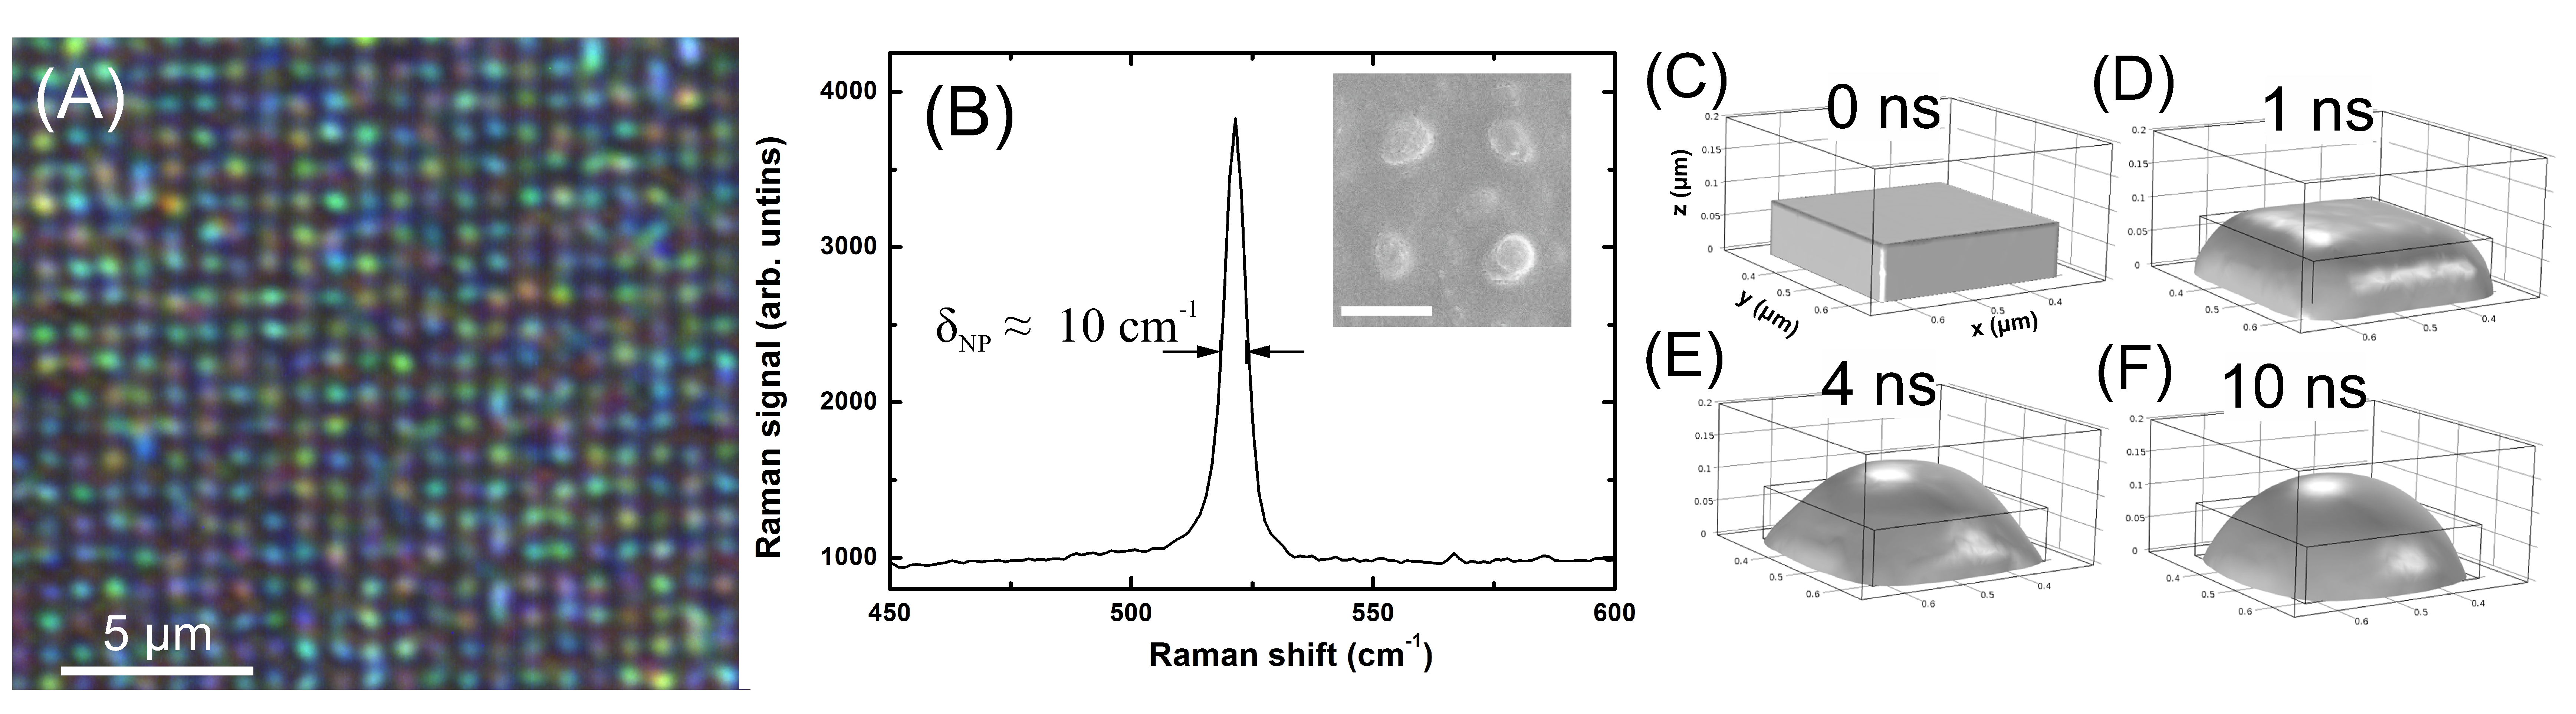
\includegraphics[width=0.9\textwidth]{figs/results/fab/LaserWriting.eps}
                    \end{center}
                    \caption{}
                    \label{fig:LaserWriting}
            \end{figure}


            As we have shown, the laser \hlb{transfer} method allows to fabricate c-Si nanoparticles with
            distinguished resonances, however it does not allow to obtain an ordered array of nanoparticles
            from the amorphous film similarly to the previously published results on bulk c-Si~\cite{zywietz2014generation}.
            Therefore, we develop a novel method of direct laser writing of c-Si resonant nanoparticles via cutting of submicron
            square patches by the fs-laser irradiation at a 80~MHz repetition rate (Fig.~\ref{fig:LaserWriting}A). At scanning velocity of
            1~mm/s and laser fluence of $\approx$ 100~mJ/cm$^{2}$, narrow (width of $\approx$300~nm) grooves can be written directly
            in the a-Si:H film.

            Under the optimal conditions of fabrication the resulting array of nanoparticles has a period of about 0.9~$\mu$m,
            exhibiting bright colors originating from the resonant scattering (Fig.~\ref{fig:LaserWriting}A). Though the cutting should
            produce an array of square patches, our SEM images show that the nanoparticles look almost circular from the top
            (Fig.~\ref{fig:LaserWriting}B). This is due to thermal isolation of the patch from the rest of the film and its overheating
            during the cutting by a train of femtosecond laser pulses with the period of 12.5~ns. These microscale patches are
            known to be unstable at high temperatures and undergo dewetting to a certain number of similar nanoparticles depending
            on their dimensions~\cite{thompson2012solid}. In order to provide deeper insight into the mechanism of the patches reshaping,
            we model the time dynamics of the cut liquid silicon patch with the height of 80~nm and similar widths of 300~nm
            (Figs.~\ref{fig:LaserWriting}C) on a fused silica substrate in the COMSOL software, solving the incompressible Navier-Stokes
            equations and taking into account the parameters of the used materials. The modeling shows that after ten nanoseconds
            the patch is transformed into the hemisphere with a height of about 140~nm and width of about 350~nm (Figs.~\ref{fig:LaserWriting}C-F),
            giving qualitative agreement with the experimentally observed shapes.

            The corresponding Raman signals from these nanoparticles also reveal the crystalline state of the nanoparticles written
            by the laser, demonstrating a narrow peak at 520~cm$^{-1}$, with a halfwidth about 10~cm$^{-1}$ (Fig.~\ref{fig:LaserWriting}B),
            which is larger than the halfwidth of the printed nanoparticles about 4--5~cm$^{-1}$. The larger halfwidth corresponds
            to the smaller mean crystallite size, i.e. less than 10~nm according to the previous studies~\cite{campbell1986effects}.
            The origin of this difference is related to the faster cooling rate for the written nanoparticles on the fused silica
            substrate as compared with nanoparticles flying in air before deposition in the \hlb{transfer} mode, owing to the 20-fold
            larger value of the glass thermal conductivity in comparison with that one for air.

        \subsubsection{\hlb{Laser Transfer of Nanoparticles}}
            \begin{figure}[!ht]
                    \begin{center}
                        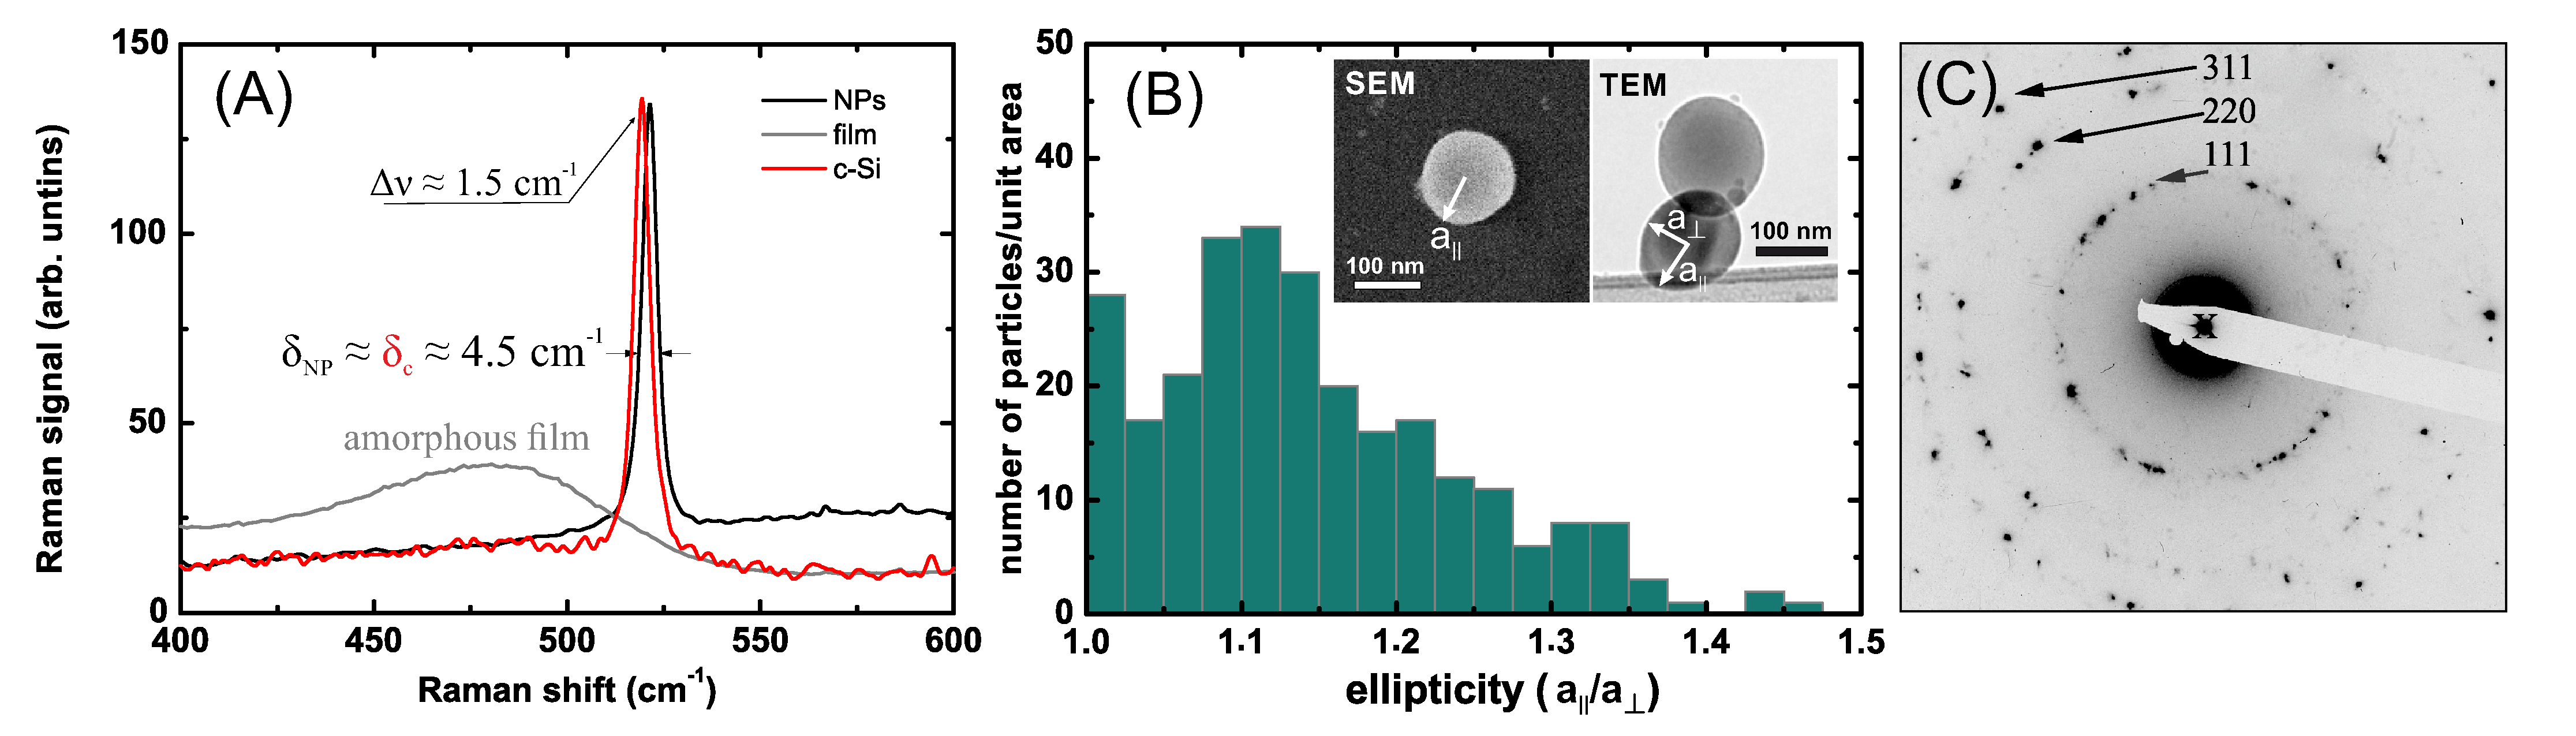
\includegraphics[width=0.9\textwidth]{figs/results/fab/Crystallinity.eps}
                    \end{center}
                    \caption{}
                    \label{fig:Crystallinity}
            \end{figure}

                We characterized the initial a-Si:H film revealing its amorphous state from the observation of its broad Raman
            peak centered around 480~cm$^{-1}$. The measured Raman spectra from individual nanoparticles have narrow peaks at
            521.5~cm$^{-1}$, corresponding to the crystalline cubic diamond structure. The reference Raman signal from a bulk
            crystalline silicon wafer and the literature data say that the Raman peak of pure crystal corresponds to 520~cm$^{-1}$.
            The slight positive shift of the peak of the nanoparticles $\Delta$$\nu$ = 1.5~cm$^{-1}$ is explained by the
            residual compressive stress~\cite{de1996micro}. Another important characteristic extracted from the Raman spectra
            is the crystallite size, which is larger than $\sim$20~nm, because the Raman peaks of the nanoparticles have
            almost the same halfwidth (4--5~cm$^{-1}$) as the peak from bulk crystalline silicon wafer (4.5~cm$^{-1}$)
            ~\cite{campbell1986effects}.

                The Raman measurements agree with characterization of the printed nanoparticles by means of transmission electron
            microscopy (TEM). \hlr{We used specimen grids (3-mm-diameter, 200-mesh copper grids, coated on one side with a 20-nm-thick
            film of amorphous carbon) to collect nanoparticles ablated from the a-Si:H film. The size, structure, and composition
            of the collected nanoparticles were determined using bright and dark field TEM imaging, see the inset in Fig.
            ~\ref{fig:Crystallinity}B. The analysis of the electron diffraction pattern from several nanoparticles shows clear maxima,
            corresponding to certain crystalline planes (Fig.~\ref{fig:Crystallinity}C). Because the specimen grids were uneven, the
            nanoparticles were deposited at different angles to the substrate meaning that TEM imaging also provides information
            on the oblateness of the particles along the direction perpendicular to the substrate surface, giving the average
            ellipticity about $a_{\parallel}/a_{\perp}\approx$1.12, where $a_{\parallel}$($a_{\perp}$) is the particle semi-major
            (semi-minor) axis oriented parallel (perpendicular) to the surface of the substrate. Indeed, scanning electron
            microscopy (SEM, Carl Zeiss, Neon 40) confirms that the particles possess \hlb{axial} symmetry along the substrate
            normal (Fig.~\ref{fig:Crystallinity}B). These results correlate with previously observed oblateness of the printed silicon
            nanoparticles~\cite{zywietz2014laser}.}

                As was reported previously~\cite{zywietz2014laser, zywietz2014generation}, the mean size of the printed nanoparticles
            strongly depends on laser fluence. In our experiments we also observed similar behaviour. In particular, two different
            regimes of the nanoparticle generation were observed. The first regime represents the gradual growth of the nanoparticle
            size with an increase of fluence up to 150~mJ/cm$^{2}$, manifesting in the change of their colors from blue to red
            (Figs.~\ref{fig:Darkfield}A--C). Such behaviour can be described in terms of the spallation mechanism of laser ablation, where
            a thin molten layer is spalled due to the laser-induced tensile pressure waves~\cite{ionin2013thermal,wu2014microscopic},
            breaking into a number of liquid droplets via the Rayleigh-Plateau instability~\cite{papageorgiou1995breakup}.
            The photomechanically spalled volume increases as V$\sim$ln(E) under the action of a Gaussian beam, owing to the
            logarithmic dependence of the spalled surface layer area r$^{2}$$_{s}$$\sim$ln(E)~\cite{bauerle2013laser}, whereas
            the thickness of the layer remains almost constant~\cite{ionin2013thermal} or even decreases~\cite{wu2014microscopic}.
            In previous studies of nanoparticle \hlb{generation} from crystalline silicon such an increase of the molten volume led
            to an increase in the number of nanoparticles~\cite{zywietz2014generation} and their size~\cite{zywietz2014laser},
            which agrees with our results (Fig.~\ref{fig:Darkfield}A--C).

                The second regime of the nanoparticle fabrication corresponds to F~$>$~150~mJ/cm$^{2}$, where large (red) nanoparticles
            are followed by small nanoparticles with a much broader size distribution (Fig.~\ref{fig:Darkfield}D). This regime is related to
            unstable boiling of superheated silicon~\cite{bulgakova2001pulsed, ionin2013thermal, wu2014microscopic}, when the
            nanoparticle formation occurs through explosive decomposition of the material into vapor and small
            clusters/droplets~\cite{itina2009molecular,wu2014microscopic}, yielding nanoparticles with the mean sizes smaller than
            100~nm~\cite{amoruso2004generation}. Small silicon nanoparticles fabrication in this regime has been extensively studied
            over last two decades~\cite{amoruso2004generation, tull2006formation} for a number of biomedical applications.
            However, one can conclude that the high-fluences regime (Fig.~\ref{fig:Darkfield}D) is not desirable for reproducible Mie-type
            nanoresonators fabrication, whereas the low-fluence regimes (Fig.~\ref{fig:Darkfield}A--C) provide much more controllable
            nanoparticle \hlb{generation and deposition}. The Raman, TEM and SEM characterization of the printed silicon nanoparticles
            helped to determine their almost perfect crystalline phase, meaning that it is possible to fabricate the crystalline
            silicon nanoresonators from amorphous films, which is very useful for low-loss all-dielectric nanophotonics.

    \subsection{\hlb{Characterization of Resonant Optical Modes of the Nanoparticles}}
        \label{sec:DarkfieldExp}


        \begin{figure}[!ht]
                \begin{center}
                    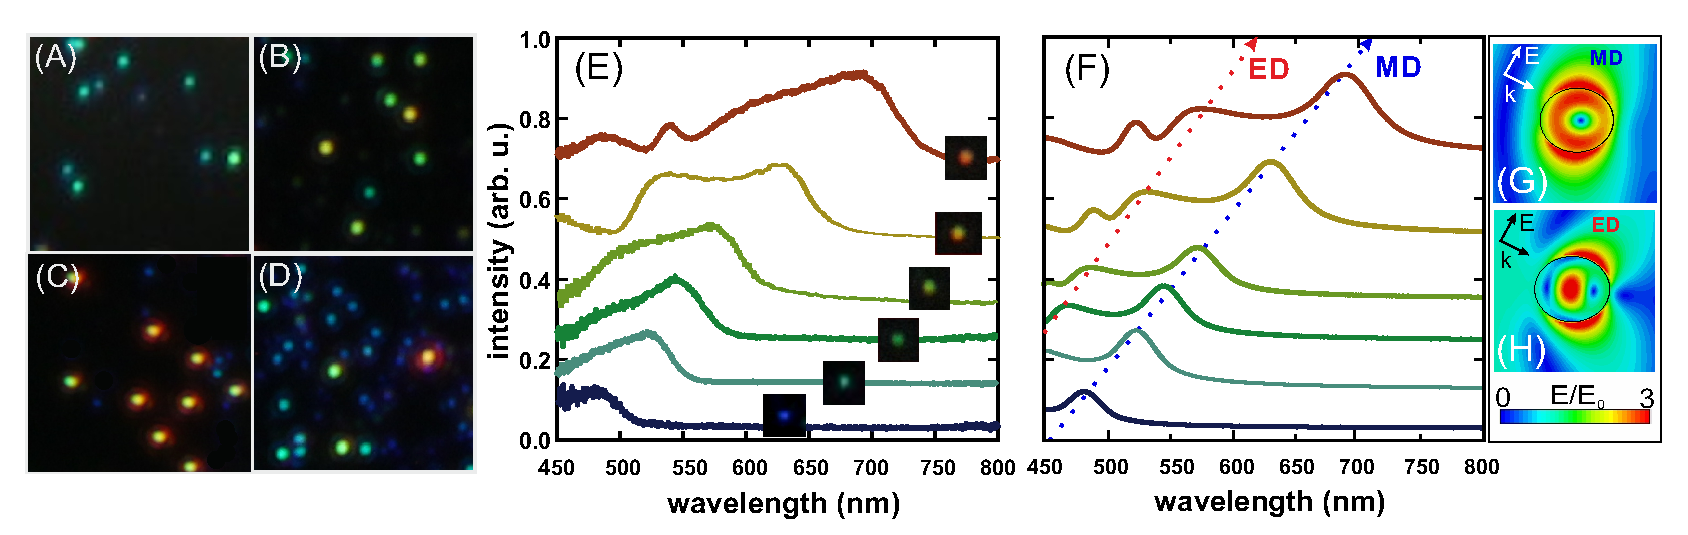
\includegraphics[width=0.9\textwidth]{figs/results/char/DarkField.eps}
                \end{center}
                \caption{Dark-field optical images of silicon nanoparticles fabricated at different peak fluences:
                120 (A), 130 (B), 140 (C), 160~mJ/cm$^{2}$ (D). Experimental (E) and theoretical (F) spectra for
                scattered p-polarized incident light (angle of incidence is 65$^{\circ}$) from individual nanoparticles
                with the radius parallel to substrate surface a$_{\parallel}$ = 55~nm (blue), 65~nm (spring green),
                68~nm (green), 72~nm (olive), 85~nm (yellow) and 92~nm (red) with the ellipticity coefficient of 1.12.
                Numerically calculated electric field distributions in the silicon nanoparticle with a$_{\perp}$ = 85~nm
                 the wavelengths of 635~nm (G) and 525~nm (H).}
                \label{fig:Darkfield}
        \end{figure}


        The excitation of the electric dipole (ED) and magnetic dipole (MD) resonances is proven by simulations
        in CST Microwave Studio. The scattering geometry is modelled as a c-Si ellipsoid with different axis
        ($a_{\perp}$ and $a_{||}$) and the fixed ellipticity $a_{\parallel}/a_{\perp}\approx$~1.12, i.e. for
        the most probable ellipticity parameter in the experiments. The ellipsoid is irradiated by a plane wave
        at the angle 65$^{\circ}$ in vacuum. Modeling of scattering spectra (Fig.~\ref{fig:Darkfield}F) shows good agreement
        with the corresponding experimental ones (Fig.~\ref{fig:Darkfield}E), whereas the modeled electric field distributions
        in the ellipsoids at different wavelengths reveal excitation of MD (Fig.~\ref{fig:Darkfield}G) and ED (Fig.~\ref{fig:Darkfield}H).

    \subsection{\hlb{Determining Size of Nanoparticle from Optical Resonance Positions}}

        \begin{figure}[!ht]
                \begin{center}
                    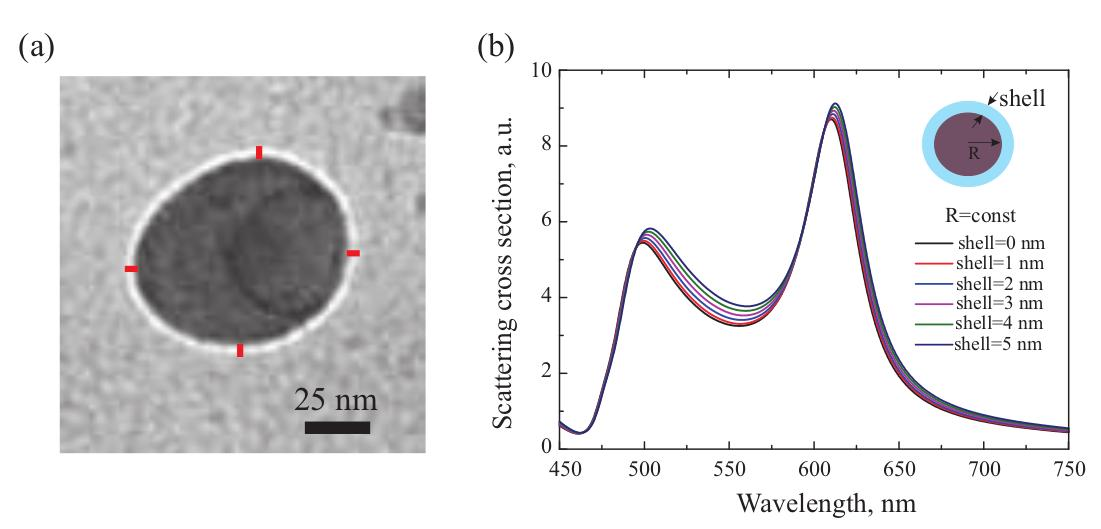
\includegraphics[width=0.9\textwidth]{figs/results/char/CoreShell.jpg}
                \end{center}
                \caption{\textbf{a}. TEM image of the typical silicon nanoparticle fabricated using laser-induced
                            forward transfer technique. Red lines represent 5 nm. \textbf{b}. Total scattering cross sections of
                            silicon nanoparticle (R = 75 nm) coated with silica layers with different thicknesses.}
                \label{fig:CoreShell}
        \end{figure}

%         Scanning electron microscopy (SEM, Carl Zeiss, Neon 40), registering backscattered electrons, was used
%     determine the geometrical parameters of the nanoparticles. In particular, that the particles possess \hlr{axial}
%     symmetry along the substrate normal (Fig.~\ref{fig:Crystallinity}B).
%     We used specimen grids (3-mm-diameter, 200-mesh copper grids, coated on one side with a 20-nm-thick film
% of amorphous carbon) to collect nanoparticles ablated from the a-Si:H film. The size, structure, and composition
% of the collected nanoparticles were determined using bright and dark field TEM imaging, see the inset in
% Fig.~\ref{fig:Crystallinity}B. The analysis of the electron diffraction pattern from several nanoparticles shows clear maxima,
% corresponding to certain crystalline planes (Fig.~\ref{fig:Crystallinity}C). \hlr{Because the specimen grids were uneven, the
% nanoparticles were deposited at different angles to the substrate meaning that} TEM imaging also provides information
% on the oblateness of the particles along the direction perpendicular to the substrate surface, giving
% the average ellipticity about $a_{\parallel}/a_{\perp}\approx$1.12, where $a_{\parallel}$($a_{\perp}$) is
% the particle semi-major (semi-minor) axis oriented parallel (perpendicular) to the surface of the substrate.



        Resonant optical properties of silicon nanoparticles are known to be sensitive to their shape[\cite{zywietz2015electromagnetic}],
        crystallinity[\cite{zywietz2015electromagnetic, dmitriev2016laser}], to the substrate[\cite{miroshnichenko2015substrate}] and
        to the thickness of native oxide layer[\cite{zywietz2015electromagnetic, fu2012directional}],
        which is always present on silicon surface[\cite{morita1990growth}]. In this work, the shape of the particles has been controlled using
        SEM measurements, while the diameter of silicon core has been extracted from dark-field spectroscopy experiments.
        In order to analyze the influence of native silicon oxide layer on the optical properties of the studied nanoparticles,
        we carried out additional experimental measurements and numerical simulations. First, to estimate the thickness of the
        layer, we have characterized typical silicon nanoparticle using transmission electron microscopy (TEM), see Fig. [\ref{fig:CoreShell}A].
        Our measurements confirm that nanoparticles are coated with less than 5-nm-thick silica layer, which is in good agreement
        with previously reported results[\cite{zywietz2015electromagnetic, fu2012directional}]. To analyze the influence of the oxide
        layer on the resonant properties of nanoparticles,
        we have simulated total scattering cross section spectra of a crystalline silicon nanoparticle (D = 150 nm) surrounded by
        silica shells with different thicknesses, see Fig. [\ref{fig:CoreShell}]. For the sake of simplicity, the simulations have been carried out
        using Mie theory[\cite{bohren1983absorption}]. Our results confirm that in the case of fixed silicon core diameter appearance of additional
        5-nm-thick silica layer leads to red spectral shifts of both electric and magnetic dipole resonances of the
        nanoparticle as small as $≈ 4.2$nm and $≈ 2.5$nm, respectively. The influence of different substrates has been analyzed in
        Ref. [\cite{miroshnichenko2015substrate}] The authors have demonstrated that both electric and magnetic dipole resonances of
        crystalline silicon nanoparticle
        placed on the fused silica substrate exhibit small red spectral shifts with respect to the resonances of the nanoparticle
        in free space. In the case of nanoparticle with the diameter of $D = 130 $nm these shifts are as small as $≈ 3.5 $nm and $≈ 0.5$ nm,
        respectively. Therefore, the spectral shift of the nanoparticle’s magnetic dipole resonance is practically insensitive to both
        the substrate and the native silica layer. This allows to conclude that the diameter of silicon core of the nanoparticle
        can be precisely extracted from the spectral position of magnetic dipole resonance in the dark-field spectroscopy measurements
        compared to the simulations based on Mie theory.


    \subsection{\hlb{Raman Scattering Enhancement from Single Nanoparticles}}
        \label{sec:RamanExp}
        Theoretically predicted enhancement of Raman scattering at different Mie-resonances was directly compared with our
        experiments with individual crystalline silicon (c-Si) nanospheres lying on a fused silica substrate (details of the
        fabrication are in \hlr{Methods}). In order to determine the resonant properties of nanoparticles, we measure
        their scattering spectra in the dark-field scheme (Fig.~\ref{fig:EnhancementExp}a, see \hlr{Methods} below).

        \begin{figure}[!ht]
            \begin{center}
                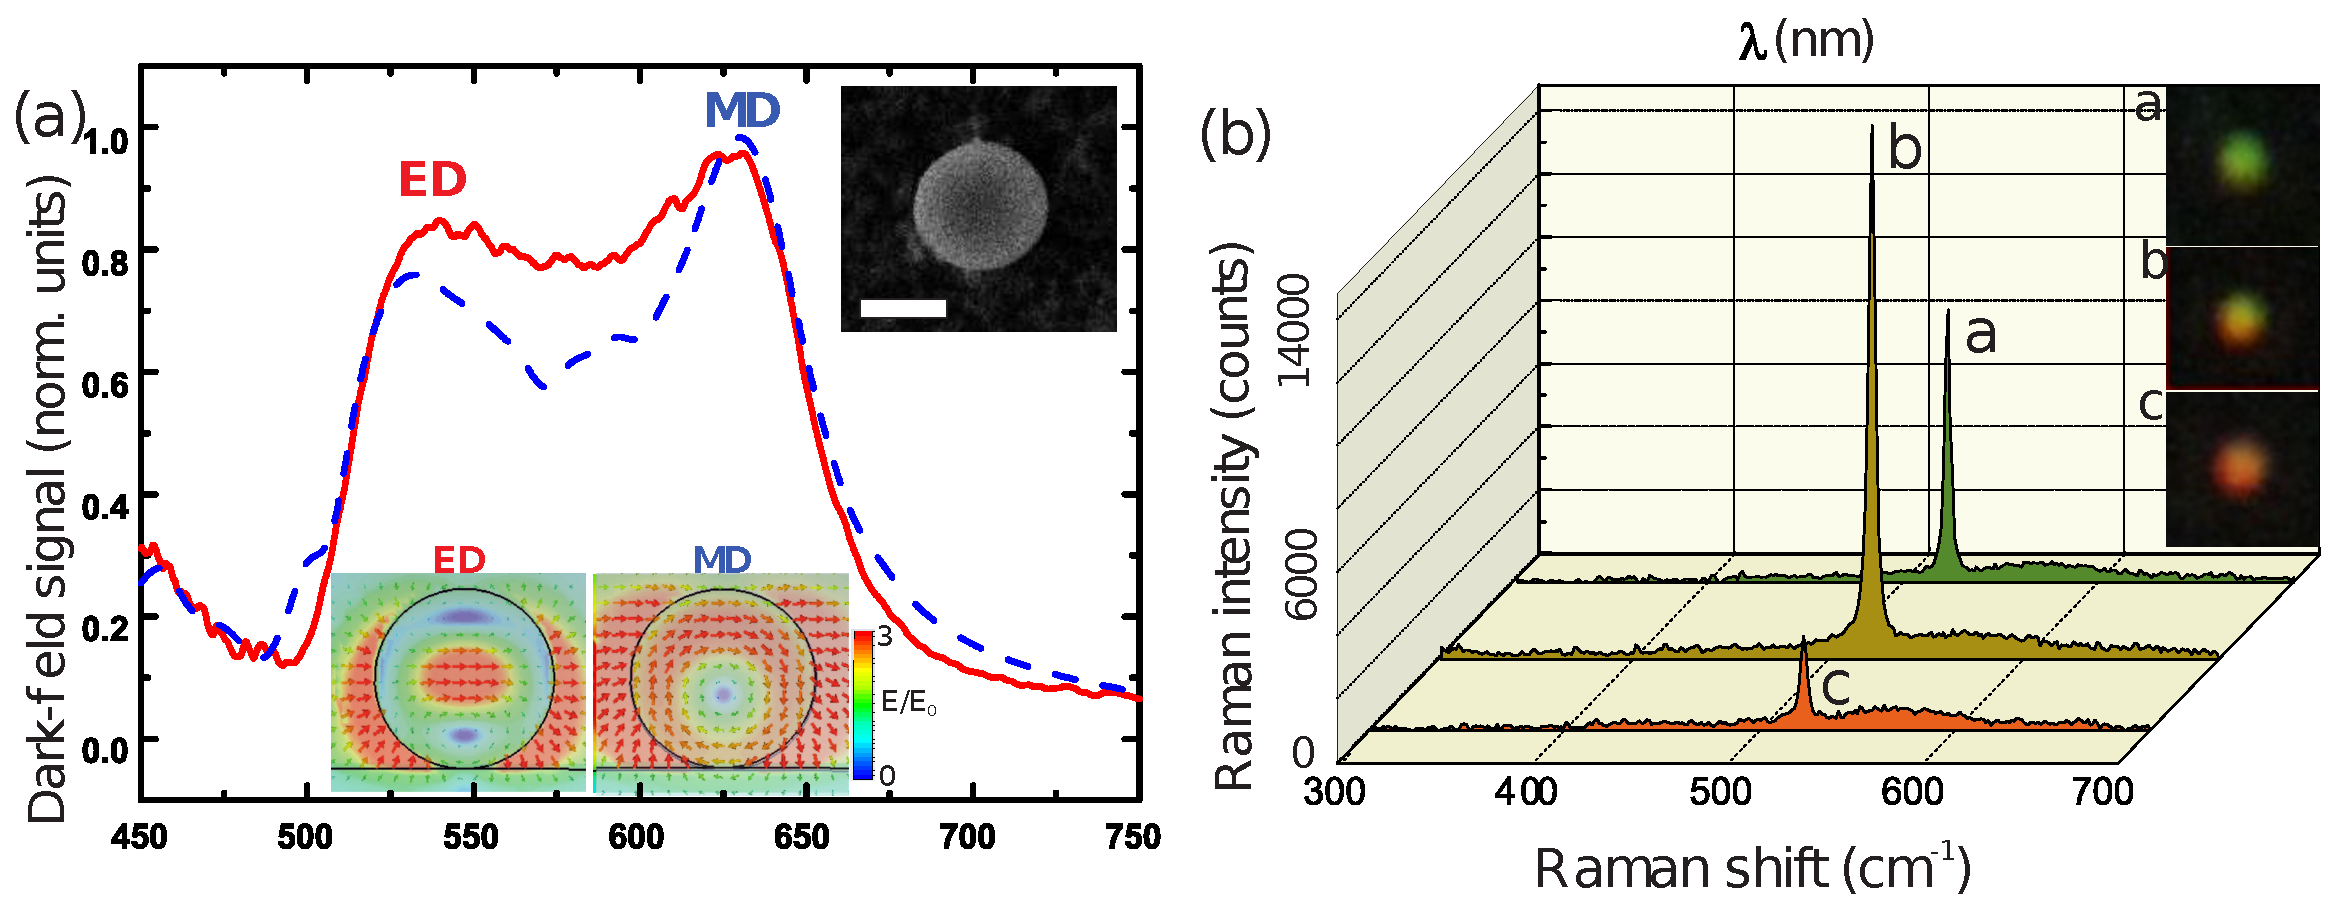
\includegraphics[width=0.9\textwidth]{figs/results/enhance/EnhancementExperiment.eps}
            \end{center}
            \caption{(\textbf{a}) Experimental (solid) and theoretical (dashed) scattering spectra for s-polarized incident light.
            Bottom inset: the electric field distribution at different wavelengths, corresponding to electric dipole (ED) and magnetic
            dipole (MD) resonances. Upper inset: SEM image of typical ablative c-Si nanoparticle (scale bar represents 100~nm). (\textbf{b})
            Raman spectra for different nanoparticles at the excitation wavelength of 633 nm and the corresponding dark-field optical images of the
            nanoparticles: (a) D=153 nm, (b) D=158 nm, (c) D=173 nm.}
            \label{fig:EnhancementExp}
        \end{figure}

        In order to confirm the excitation of ED and MD resonances, we simulate numerically the scattering spectra by the method of
        discrete-dipole approximation (DDA) and analyze near fields by the full-wave modeling in CST Microwave Studio (for details of
        these calculations see \hlb{Methods}). The results of numerical modeling are shown in Fig.~\ref{fig:EnhancementExp}a, and they exhibit a
        good agreement with experimental results, revealing the mode structure at each spectral maximum. We use optical properties for
        c-Si from Ref.~\cite{vuye1993temperature}, giving the best fitting of our experimental scattering spectra. Minor differences of the results in
        the region of 550--600~nm may be attributed to the presence of a SiO$_2$ substrate.

        \begin{figure}[!hb]
            \begin{center}
                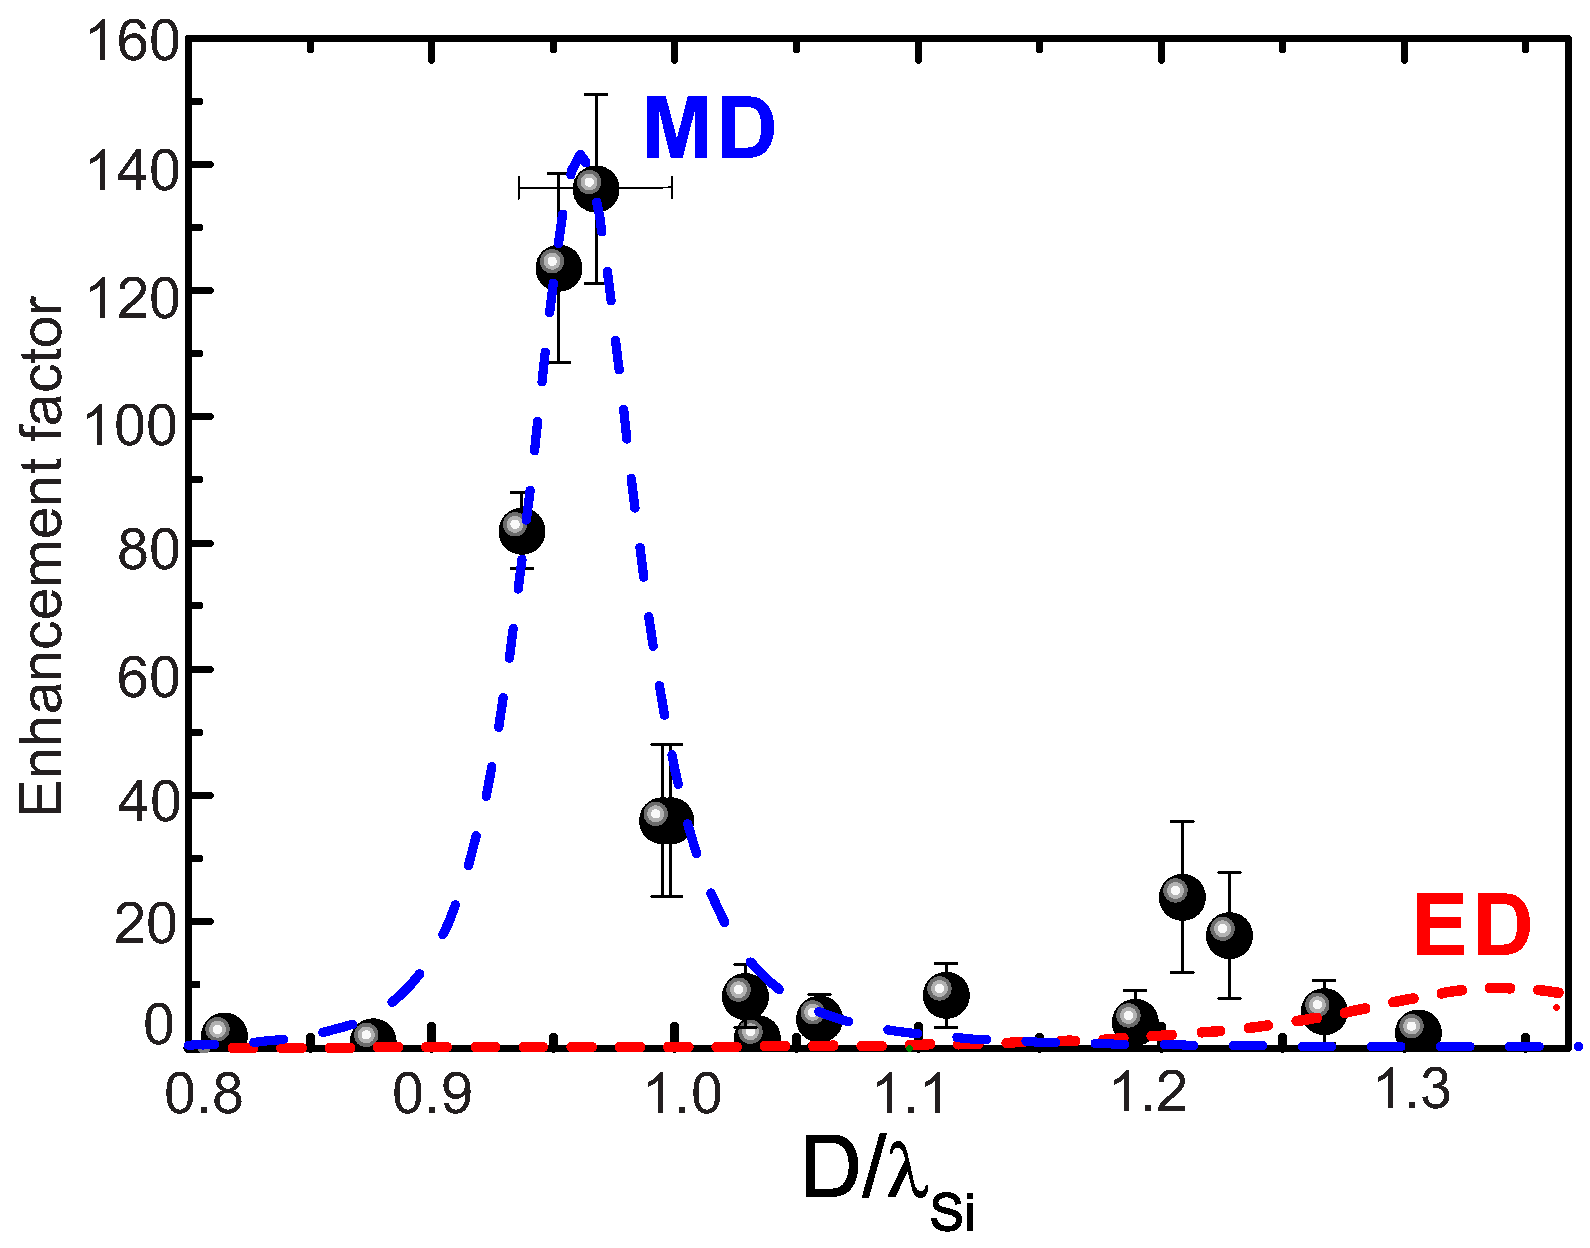
\includegraphics[width=0.5\textwidth]{figs/results/enhance/EnhancementExperimentTheory.eps}
            \end{center}
            \caption{Theoretical (dashed curves) and experimental (black dots) dependencies of the enhancement factor for Raman
            scattering from spherical silicon nanoparticles on their diameter D normalized to the excitation wavelength in silicon.
            Theoretical dependence consists of two contributions from magnetic dipole (blue dashed curve) and electric dipole
            (red dashed curve).}
            \label{fig:EnhancementExpTheory}
        \end{figure}

        The measured Raman scattering signal from individual nanoparticles exhibits extremely strong dependence on their size
        and color in the dark-field images (Fig.~\ref{fig:EnhancementExp}b). Such a dependence for the excitation light at the wavelength
        $\lambda$=633~nm shows a maximum of Raman scattering for nanoparticles with $D\approx 155$~nm, supporting MD resonance
        at this wavelength. The maximum value of the enhancement factor (EF) for nanoparticles with MD in comparison with
        nanoparticles with diameters $D\approx125$~nm and $D\approx175$~nm is about $EF\approx$140. The calculation of EF
        from experimental data is based on the formula: EF~=~(I/I$_{\rm norm}$)$\times$(V/V$_{\rm norm}$), where I is Raman
        scattering signal from a studied nanoparticle with known diameter and volume V, I$_{\rm norm}$ is Raman signal from
        a nanoparticle of known volume V$_{\rm norm}$ with the smallest observed signal. To make such a normalization, the
        nanoparticle with $D\approx$135~nm is chosen. In order to check the effect of excitation wavelength, we also measured
        the Raman spectra at $\lambda$=532~nm for the same nanoparticles. Here, the maximum EF values observed for nanoparticles
         are relatively small at $\lambda$=633~nm, i.e. for diameters around 125~nm and 175~nm.

        In order to distinguish contributions from each type of Mie resonances, the generalized EF dependence of Raman
        scattering should be represented in terms of the dimensionless nanoparticle diameter $D/\lambda_{\rm Si}$,
        taking into account different refractive indices at different wavelengths (Fig.~\ref{fig:EnhancementExpTheory}). Such a dependence
        exhibits a pronounced maximum with a peak $EF\approx$140 at D/$\lambda_{\rm Si}$ $\approx$ 1, i.e. near the
        magnetic dipole resonance. This value is 5-7 times larger than EF for the electric dipole. Insets in Fig.~\ref{fig:EnhancementExp}a
        provide an illustrative interpretation of this enhancement. At the MD resonance, a larger farction of electromagnetic
        energy is stored inside the nanoparticle, thus increasing total Raman polarization and emission.
        Corresponding theoretical calculations for perfect spherical c-Si nanoparticles predict even larger difference between
        MD and ED ($\sim$ 10), which is not perfectly matched with our observations owing to the existence of nanoscale
        deviations and few-nm natural oxide layer~\cite{fu2012directional, zywietz2015electromagnetic}. Nevertheless, the
        Raman signal enhancement in the vicinity of MD is in excellent agreement with our model. The data shown in Fig.~\ref{fig:EnhancementExpTheory}
        is limited to nanoparticle diameters $D/\lambda_{\rm Si}<1.3$ as our fabrication method does not allow to make larger
        particles without pronounced ellipticity. At the same time, even small deviation from the spherical shape leads to
        suppression of the MQ resonance~\cite{fu2012directional}.
